<<<<<<< HEAD
\chapter{\textcolor{orange}{SRS - SOFTWARE REQUERIMENTS SPECIFICATION}}
=======
\chapter{\textcolor[gray]{.2}{SRS - SOFTWARE REQUERIMENTS SPECIFICATION}}
>>>>>>> 3910ab7b9e4c32b7e12f785ce015e1bd7260973a

%\newpage
%\section{\textcolor{orange}{Historial de Versiones}}
%\begin{table}[H]
%\begin{center}
%\begin{tabular}{|c|c|c|c|}
%\hline
%\rowcolor[RGB]{255,127,0} Vesión & Fecha & Descripción de Cambios & Autor\\
%\hline
%1.0 & 09/07/2013 & Primera Versión & Gomez P.\\
%\hline
%1.1 & 01/12/2013 & LEL, Escenarios y Tarjetas CRC & Lovaisa V.\\
%\hline

%\end{tabular}
%\end{center}
%\end{table}
%\newpage

<<<<<<< HEAD
=======
\newpage
\section{\textcolor[gray]{.2}{Historial de Versiones}}
\begin{table}[h!]
\begin{center}
\begin{tabular}{|c|c|c|c|}
\hline
\rowcolor[gray]{.8} Vesión & Fecha & Descripción de Cambios & Autor\\
\hline
1.0 & 09/07/2013 & Primera Versión & Gomez P.\\
\hline
1.1 & 01/12/2013 & LEL, Escenarios y Tarjetas CRC & Lovaisa V.\\
\hline
\end{tabular}
\end{center}
\end{table}
>>>>>>> 3910ab7b9e4c32b7e12f785ce015e1bd7260973a

%\section{\textcolor{orange}{Página de Aprobaciones}}
%A continuación se listan las personas de las cuales se requiere la aceptación de cualquier cambio mayor de este documento.
%\begin{enumerate}
 % \item Estas aprobaciones no son necesarias si el cambio es menor.
 % \item Estas aprobaciones son necesarias si el cambio es realizado por alguna persona distinta de ellas.
%\end{enumerate}
%\begin{table}[h!]
%\begin{center}
%\begin{tabular}{|c|c|c|c|}
%\hline
%\rowcolor[RGB]{255,127,0} Nombre & Cargo & Fecha & Firma\\
%\hline
%Lovaisa Valeria & Resp. Ingeniería de Requerimientos & 09/07/2013 & \\
%\hline
%Gomez Pablo & Resp. Suplente & 09/07/2013 & \\
%\hline
%\end{tabular}
%\end{center}
%\end{table}

<<<<<<< HEAD

%\newpage

\section{\textcolor{orange}{Introducción}}
\subsection{\textcolor{orange}{Propósito y Alcance}}
=======
\section{\textcolor[gray]{.2}{Página de Aprobaciones}}
A continuación se listan las personas de las cuales se requiere la aceptación de cualquier cambio mayor de este documento.
\begin{enumerate}
  \item Estas aprobaciones no son necesarias si el cambio es menor.
  \item Estas aprobaciones son necesarias si el cambio es realizado por alguna
  persona distinta de ellas.
\end{enumerate}
\begin{table}[h!]
\begin{center}
\begin{tabular}{|c|c|c|c|}
\hline
\rowcolor[gray]{.8} Nombre & Cargo & Fecha & Firma\\
\hline
Lovaisa Valeria & Resp. Ingeniería de Requerimientos & 09/07/2013 & \\
\hline
Gomez Pablo & Resp. Suplente & 09/07/2013 & \\
\hline
\end{tabular}
\end{center}
\end{table}


\newpage
\section{\textcolor[gray]{.2}{Introducción}}
\subsection{\textcolor[gray]{.2}{Propósito y Alcance}}

>>>>>>> 3910ab7b9e4c32b7e12f785ce015e1bd7260973a
Este documento cubre el proceso de elicitación de requerimientos del sistema
de monitoreo y registro de datos multipropósito. Este SRS tiene como objetivo
establecer cuales son los requerimientos del sistema a nivel de usuario, como
así también a nivel de sistema (requerimientos detallados). 

\subsection{\textcolor[gray]{.2}{Acrónimos y Glosario}}
\begin{table}[h!]
\begin{center}
\begin{tabular}{|c|c|}
\hline
\rowcolor[gray]{.8} Acrónimo & Descripción \\
\hline
SRS & Software Requirements Specification - Especificación de Req. de Software \\
\hline
SRM & Software Requirements  Manager – Responsable de requerimientos del sistema\\
\hline
\end{tabular}
\end{center}
\end{table}

\subsection{\textcolor[gray]{.2}{Herramientas Necesarios}}
\begin{table}[h!]
\begin{center}
\begin{tabular}{|c|p{100mm}|}
\hline
\rowcolor[gray]{.8} Programa & Propósito \\
\hline
Planilla de Cálculos Generica & Para llevar en control de la trazabilidad
de requermientos usr. vs req. de sistema y de req. vs casos de uso.\\
\hline
Dia & Software para la creación de diagramas UML\\
\hline
Google-Drive & Software necesario para llevar el control de los requerimientos.\\
\hline
\end{tabular}
\end{center}
\end{table}

%\newpage
%\\section{\\textcolor[gray]{.2}{Roles}}
%\subsection{\textcolor[gray]{.2}{Responsables}}
%Las actividades de ingeniería de requerimientos del Sistema serán coordinadas en este proyecto por el Responsable de Requerimientos del sistema. (SRM). Este Rol debe ser asignado a alguno de los miembros del proyecto.
%El SRM será el responsable directo de las actividades de requerimientos del
%sistema, responder ante modificaciones en los mismos  y de mantener la documentación relacionada actualizada (Modificación de requerimientos , Modificación del sistema de trackeo).

%\subsection{\textcolor[gray]{.2}{Roles}}
%\begin{table}[!h]
%\begin{center}
%\begin{tabular}{|c|c|c|}
%\hline
%\rowcolor[gray]{.8} Rol & Nombre & Suplente\\
%\hline
%SRM & Lovaisa Valeria & Gomez Pablo\\
%\hline
%\end{tabular}
%\end{center}
%\end{table}

\newpage
\section{\textcolor[gray]{.2}{Requerimientos}}
\subsection{\textcolor[gray]{.2}{Listado de Requerimientos No Funcionales}}
\subsubsection{\textcolor[gray]{.2}{Requerimientos de apariencia
(Requerimientos de percepción)}}
\begin{enumerate}
\item Las interfaces gráficas deben estar elaboradas bajo el Framework Qt
\item El sistema debe brindar una interfaz gráfica basada en ventanas ,
formularios y menues.
\item El sistema debe visualizarse en Español (Latinoamérica – Argentina).
\end{enumerate}


\subsubsection{\textcolor[gray]{.2}{Requerimientos de facilidad de utilización
(Requerimientos de usabilidad)}}
\begin{enumerate}
\item El sistema debe permitir el teclado como dispositivo de entrada.
\item El sistema debe permitir el mouse como dispositivo de entrada.
\end{enumerate}

\subsubsection{\textcolor[gray]{.2}{Requerimientos de velocidad y latencia
(Requerimientos de desempeño)}}
\begin{enumerate}
\item El sistema debe tener un tiempo de respuesta menor o igual a un (1)
segundo.
\item El sistema debe tener acceso a una red LAN Ethernet de velocidad 100 Mbps.
\end{enumerate}

\subsubsection{\textcolor[gray]{.2}{Requerimientos de confiabilidad y
disponibilidad (Requerimientos de desempeño)}}
\begin{enumerate}
\item El sistema debe estar disponible mínimo un 99\% del tiempo en el que este
se encuentre en ejecución.
\end{enumerate}

\subsubsection{\textcolor[gray]{.2}{Requerimientos de capacidad (Requerimientos de
desempeño)}}
\begin{enumerate}
\item El sistema debe tener acceso a mínimo 512 KB de memoria RAM disponibles
para la ejecución de su módulo de presentación gráfica.
\item El sistema debe tener acceso a mínimo 512 KB de memoria RAM disponibles
para la ejecución de su módulo de manejo y registro de datos.
\item El sistema debe tener acceso a mínimo un procesador de 1 GHz para la
ejecución de su módulo de presentación gráfica.
\item El sistema debe tener acceso a mínimo un procesador de 1.2 GHz para la
ejecución de su módulo de manejo y registro de datos.
\end{enumerate}
 
\subsubsection{\textcolor[gray]{.2}{Requerimientos de ambiente físico esperado
(Requerimientos operacionales y ambientales)}}
\begin{enumerate}
\item El módulo de adquisición de datos debe poder ejecutarse un
microcontrolador arduino MEGA2560 situado fisicamente en sala de ambiente
controlado (Valores sensados : Humedad y Temperatura).
\item El módulo de manejo y registro de datos debe poder ejecutarse en un
servidor de arquitectura x86.
\item El módulo de presentación de datos debe poder ejecutarse en una placa de
desarrollo iMx53 situada fisicamente en un lugar de facil acceso en sala de
ambiente controlado.
\end{enumerate}

\subsubsection{\textcolor[gray]{.2}{Requerimientos de acceso (Requerimientos de
seguridad)}}
\begin{enumerate}
\item El sistema debe registringir el acceso al módulo de manejo y registro de
datos en el servidor mediante usuario y contraseña. 
\item El sistema debe contar con diferentes niveles de privilegios en el acceso
a los módulos de presentación de datos y manejo/registro de datos.
\end{enumerate}

\subsubsection{\textcolor[gray]{.2}{Requerimientos de integridad (Requerimientos
de seguridad)}}
\begin{enumerate}
\item El sistema no debería permitir la modificiación de variables de
configuración durante la adquisición de datos.
\end{enumerate}

\subsubsection{\textcolor[gray]{.2}{Requerimientos de privacidad (Requerimientos
de seguridad)}}
\begin{enumerate}
\item El sistema debería guardar los datos de acceso (usuario y contraseña) en
el equipo en que se esta ejecutando. 
\end{enumerate}

\subsubsection{\textcolor[gray]{.2}{Requerimientos de inmunidad
(Requerimientos de seguridad)}}
\begin{enumerate}
\item El sistema deberá verificar que todos los datos que el usuario ingrese
sean correctos.
\item El sistema deberá verificar que todos los datos que el administrador
ingrese sean correctos.
\end{enumerate}

\subsubsection{\textcolor[gray]{.2}{Requerimientos de cumplimiento
(Requerimientos legales)}}
\begin{enumerate}
\item El sistema debe ser entregado en la semana del 22 al 26 de Julio.
\end{enumerate}


\subsubsection{\textcolor[gray]{.2}{Requerimientos de legalidad (Requerimientos
legales)}}
\begin{enumerate}
\item El sistema no puede desarrollarse bajo herramientas obtenidas de forma
ilegal (Uso de seriales copiados, cracks, keygens, entre otros)
\end{enumerate}

\subsubsection{\textcolor[gray]{.2}{Requerimientos de estándares (Requerimientos
legales)}}
\begin{enumerate}
\item El código fuente del sistema debe estar debidamente documentado en
Español (Latinoamérica – Argentina)
\item El código debe ser desarrollado en C , C++ , Qt, mysql y debe seguir los
estándares involucrados en dicha tarea.
\end{enumerate}


\newpage
\section{\textcolor[gray]{.2}{Listado de Requerimientos Funcionales}}
El listado completo de requerimientos se encuentra gestionado en una planilla de
cálculo opensource en Google Drive.


\begin{table}[h!]
\begin{center}
\begin{tabular}{|c|p{100mm}|}
\hline
\rowcolor[gray]{.8} Descripción & Link \\
\hline
Listado Maestro de Requerimientos &
\url{https://docs.google.com/spreadsheet/ccc?key=0AuDVazeuJzKkdGN2bUZoVmRlM3EybHUwVS1zWXNWTlE#gid=0}\\
\hline
\end{tabular}
\end{center}
\end{table}

Con esta herramienta se realiza la documentación de todos los requerimientos
del sistema y la gestión de modificaciones en los mismos. Así también se logra
distribuir la planificación de trabajo logrando saber quien esta desarrollando
la implementación de cada uno de estos requerimientos en ese momento.
Los requerimientos de funcionales de usuario de dividen en grupos , como
muestra la siguiente tabla.

\begin{table}[h!]
\begin{center}
\begin{tabular}{|c|c|}
\hline
\rowcolor[gray]{.8} Tipo & Descripción \\
\hline
Adquisición & Req. relacionados a la forma de obtención de los
datos.\\
\hline
Manejo y Registro & Req. relacionados a la forma en que el servidor administra
los datos\\
\hline
Presentación & Req. relacionados a la forma en que se muestran los datos al
usuario.\\
\hline
\end{tabular}
\end{center}
\end{table}

En la herramienta de gestión de requerimientos se colocarán los tags
correspondientes para cada tipo de requerimientos.
%Las asociaciones entre requerimientos y requerimientos se encuentran
%documentados en la matriz de trazabilidad.

%\begin{table}[!h]
%\begin{center}
%\begin{tabular}{|c|p{100mm}|}
%\hline
%\rowcolor[gray]{.8} Descripción & Link \\
%\hline
%Matriz de Req vs Req &
%\url{https://docs.google.com/spreadsheet/ccc?key=0AuDVazeuJzKkdFJEbkpaVV91el9EM0NSMVFYendXdWc#gid=0}\\
%\hline
%\end{tabular}
%\end{center}
%\end{table}

Las asociaciones entre diagramas de casos de uso y requerimientos se encuentran
documentados en la herramienta de gestión de requerimientos. 

%\begin{table}[!h]
%\begin{center}
%\begin{tabular}{|c|p{100mm}|}
%\hline
%\rowcolor[gray]{.8} Descripción & Link \\
%\hline
%Matriz de Req vs UCs &
%\url{https://docs.google.com/spreadsheet/ccc?key=0AuDVazeuJzKkdHR3Mm5sQUpXYldUOTlHT0JIX1l6bWc#gid=0}\\
%\hline
%\end{tabular}
%\end{center}
%\end{table}

\newpage
\subsection{\textcolor[gray]{.2}{Tabla de requerimientos - Lista maestra de
requerimientos}} 
\begin{table}[h!]
\begin{center}
\begin{tabular}{|p{30mm}|p{70mm}|p{30mm}|}
\hline
\rowcolor[gray]{.8} Requerimiento N & Descripción & Tipo \\
\hline
RQX001 & El arduino mega 2560 debe poder enviar datos tomados desde el sensor
de temperatura y humedad al servidor por medio de una conexión serial  u
Ethernet & Adquisición\\
\hline
RQX002 & El sistema de adquisición y registro de datos de temperatura debe poder
capturar datos con un intervalo máximo de 1 segundo & Adquisición \\
\hline
RQX003 & Los parámetros de configuración del modulo de Adquisición deben poder
configurarse desde el servidor de manejo y registro de datos & Adquisición \\
\hline
RQX004 & El modulo de adquisición debe poder identificarse con el servidor para
iniciar el envió de datos & Adquisición \\
\hline
RQX005 & El sistema de manejo y registro de datos debe poder conectarse con uno
o varios modulos de adquisicion de datos por medio de una conexión serial u
Ethernet & Manejo y Registro \\
\hline
RQX006 & El sistema de registro y manejo de datos de temperatura debe poder
manupular los  datos convirtiendolos a un formato legible para seres humanos &
Manejo y Registro\\
\hline
RQX007 & El sistema de registro y manejo de datos de temperatura debe poder
registrar y administrar todos los dispocitivos de adquisicion que se identifican
& Manejo y Registro\\
\hline
RQX008 & El sistema de registro y manejo de datos de temperatura debe poder
almacenar los datos recibidos y convertidos en una base de datos My SQL & Manejo
y Registro\\
\hline
RQX009 & El sistema de registro y manejo de datos de temperatura debe poder
registrar en una base de datos todos los dispocitivos de adquision que se
conecten al servidor & Manejo y Registro \\
\hline
RQX010 & El sistema de registro y manejo de datos de temperatura debe poder 
enviar via conexión Ethernet cada 1 segundo los datos al modulo de presentacion
& Manejo y Registro\\
\hline
\end{tabular}
\end{center}
\end{table}

\newpage

\begin{table}[h!]
\begin{center}
\begin{tabular}{|p{30mm}|p{70mm}|p{30mm}|}
\hline
\rowcolor[gray]{.8} Requerimiento N & Descripción & Tipo \\
\hline
RQX011 & El sistema de registro y manejo de datos de temperatura debe poder
enviar el promedió para diferentes intervalos de tiempo últimos 5, 15 y 60
minutos al modulo de presentación & Manejo y Registro\\
\hline
RQX012 & El sistema de registro y manejo de datos de temperatura debe poder
verificar los valores medidos se encuentren dentro de el rango establecido &
Manejo y Registro\\
\hline
RQX013 & El sistema de registro y manejo de datos de temperatura debe permitir
configuar los valores maximos y minimos & Manejo y Registro\\
\hline
RQX020 & El modulo de registro y manejo de datos de temperatura debe permitir a
un usuario adquierir privilegios de administrador mediante un password & Manejo
y Registro\\
\hline
RQX014 & El modulo de presentacion de datos debe poder conectarse con un
servidor via conecxion Ethernet & Presentación\\
\hline
RQX015 &  El modulo de presentacion de datos debe poder mostrar los datos de
temperatura enviados desde el servidor en al menos dos escalas distintas celsius
y farenheit & Presentación\\
\hline
RQX016 & El modulo de presentacion de datos debe poder indicar graficamente si
los valores de temperatura se encuentran fuera del rango permitido &
Presentación\\
\hline
RQX017 & El modulo de presentacion de datos debe permitir cambiar la direccion
ip del servidor & Presentación\\
\hline
RQX018 & El modulo de presentación de datos debe permitir a un administrador
seleccionar algún dispositivo de adquisición de datos conectado al servidor &
Presentación\\
\hline
RQX019 & El modulo de presentación de datos debe permitir a un administrador
acceder a las configuraciones por medio de usuario y contraseña & Presentación\\
\hline
\end{tabular}
\end{center}
\end{table}

\newpage
\subsection{\textcolor[gray]{.2}{Diagramas de Secuencia}}
\subsubsection{\textcolor[gray]{.2}{Adquisición, registro de datos y presentación de datos}}
% === Figura ====
\begin{figure}[h!]
 \begin{center}
  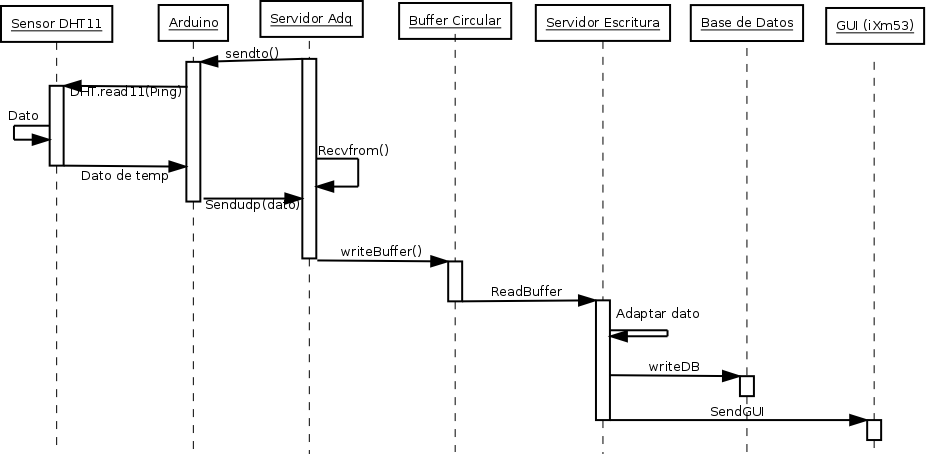
\includegraphics[width=1\textwidth,keepaspectratio=true]{img/Diagrama_secuencia.png}
  \caption{Adquisición y Registro de Datos}
  \label{fig:esquema}
 \end{center}
\end{figure}
% ===============
\subsubsection{\textcolor[gray]{.2}{Registro de nuevo dipositivo de aquisición}}
% === Figura ====
\begin{figure}[h!]
 \begin{center}
  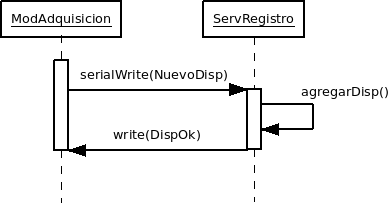
\includegraphics[width=0.5\textwidth,keepaspectratio=true]{img/agregardisp.png}
  \caption{Registro de Nuevo Dispositivo de Adquisición}
  \label{fig:esquema}
 \end{center}
\end{figure}

\newpage
\subsection{\textcolor[gray]{.2}{Diagramas de Actividades}}
% === Figura ====
\begin{figure}[h!]
 \begin{center}
  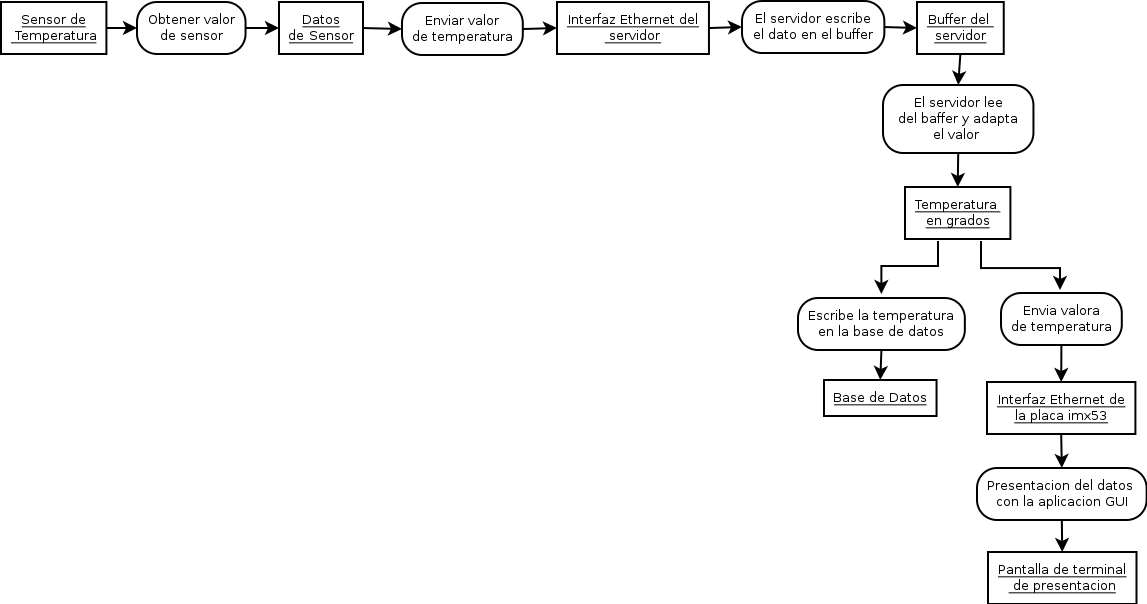
\includegraphics[width=1\textwidth,keepaspectratio=true]{img/diagactiv.png}
 \caption{Flujo de Dato de Temperatura del Sistema}
  \label{fig:esquema}
 \end{center}
\end{figure}


\subsection{\textcolor[gray]{.2}{Diagramas de Casos de Uso}}
\begin{figure}[h!]
 \begin{center}
  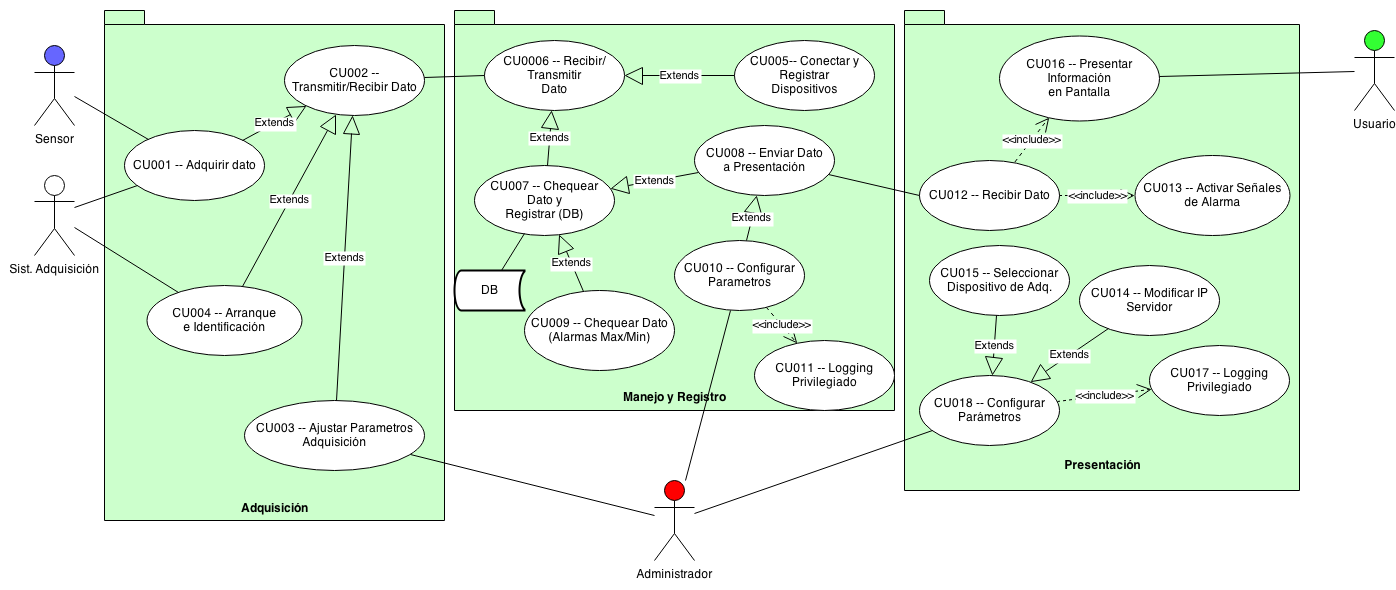
\includegraphics[width=1\textwidth,keepaspectratio=true]{img/usecases.png}
  \caption{Diagrama General de Casos de Uso}
  \label{fig:esquema}
 \end{center}
\end{figure}

\newpage
\subsection{\textcolor[gray]{.2}{LEL – Léxico Extendido del Lenguaje}}
	
		\begin{table}[h!]
		\centering
		\begin{tabular}{>{\columncolor[gray]{.8}} p{4cm} |p{9.5cm} }
		\hline
		Sinónimo  & Sensor DTH  \\
		\hline
		Noción & Entidad que adquiere y envía datos \\
		\hline
		Impacto & Envía datos al sistema de adquisición en respuesta a una solicitud \\
		\hline
		\end{tabular}
		\caption{Entrada de LEL :  Sensor DTH }
		%\label{tab:requsr1}
		\end{table}

\begin{table}[h!]
		\centering
		\begin{tabular}{>{\columncolor[gray]{.8}} p{4cm} |p{9.5cm} }
		\hline 
		Sinónimo  & Sistema de adquisición  \\
		\hline
		Noción & Entidad que solicita, recibe y envía datos \\
		\hline
		Impacto & \begin{itemize}
					 \item Solicita datos al sensor  
					 \item Recibe datos del sensor 
					 \item Establece conexión con el servidor
					 \item Envía datos al sistema de manejo y registro de datos en respuesta a una solicitud
					\end{itemize}\\
		\hline
		\end{tabular}
		\caption{Entrada de LEL : Sistema de adquisición}
		%\label{tab:requsr1}
		\end{table}

\begin{table}[h!]
		\centering
		\begin{tabular}{>{\columncolor[gray]{.8}} p{4cm} |p{9.5cm} }
		\hline
		Sinónimo  & Sistema de manejo y registro de datos  \\
		\hline
		Noción & Entidad que recibe, convierte, almacena y reenvía datos  \\
		\hline
		Impacto & \begin{itemize}
					 \item Solicita datos al sistema de adquisición   
					 \item Recibe datos del sistema de adquisición
					\item  Almacena datos en su base de datos
					 \item Establece conexión con el sistema de adquisición y el sistema de presentación de datos
					 \item Envía datos al sistema de presentación de datos en respuesta a una solicitud
					\end{itemize}\\ 
		\hline
		\end{tabular}
		\caption{Entrada de LEL :  Sistema de manejo y registro de datos }
		%\label{tab:requsr1}
		\end{table}

\newpage
\begin{table}[h!]
		\centering
		\begin{tabular}{>{\columncolor[gray]{.8}} p{4cm} |p{9.5cm} }
		\hline
		Sinónimo  & Sistema de presentación de datos  \\
		\hline
		Noción & Entidad que recibe, convierte, almacena y reenvía datos  \\
		\hline
		Impacto & \begin{itemize}
					 \item Solicita datos al sistema de manejo y registro   
					 \item Recibe datos del sistema de manejo y registro
					 \item Establece conexión con el sistema de manejo y registro de datos
					 \item Envía condiciones de alarmas al sistema de registro y manejo de datos.
					\end{itemize}\\ 
		\hline
		\end{tabular}
		\caption{Entrada de LEL : Sistema de manejo y registro de datos}
		%\label{tab:requsr1}
		\end{table}

		\begin{table}[h!]
		\centering
		\begin{tabular}{>{\columncolor[gray]{.8}} p{4cm} |p{9.5cm} }
		\hline
		Sinónimo  & Usuario  \\
		\hline
		Noción &   Entidad que consulta datos en el sistema de presentación\\
		\hline
		Impacto & 	\begin{itemize}
						\item Visualiza datos en el módulo de presentación
						\item Visualiza señales de alarma ante datos fuera de rango
					\end{itemize}\\
		\hline
		\end{tabular}
		\caption{Entrada de LEL : Usuario}
		%\label{tab:requsr1}
		\end{table}


		\begin{table}[h!]
		\centering
		\begin{tabular}{>{\columncolor[gray]{.8}} p{4cm} |p{9.5cm} }
		\hline
		Sinónimo  & Administrador  \\
		\hline
		Noción &   Entidad que configura los sistemas de adquisición, manejo \& registro y presentación de datos\\
		\hline
		Impacto & 	\begin{itemize}
						\item Ajusta parámetros de adquisición : Intervalo de adquisición , sensores conectados, etc.
						\item Configura parámetros de manejo y registro: Ajusta unidades de medida registrada, intervalo de registro , etc.
						\item Establece parámetros de presentación: Puntos máximos y mínimos de alarmas, unidad de medida presentada, sensores presentados, etc.
					\end{itemize}\\
		\hline
		\end{tabular}
		\caption{Entrada de LEL : Administrador}
		%\label{tab:requsr1}
		\end{table}


\newpage
\subsection{\textcolor[gray]{.2}{Escenarios}}

		\begin{table}[h!]
		\centering
		\begin{tabular}{>{\columncolor[gray]{.8}} p{4cm} |p{9.5cm} }
		\hline
		Título  & Adquirir dato\\
		\hline
		Objetivo &  Adquirir dato del sensor al módulo de adquisición presente en Arduino \\
		\hline
		Contexto & Conexión establecida entre el sensor y el sistema de adquisición\\
		\hline
		Recursos &  Sensor y Arduino (Módulo de adquisición)\\
		\hline
		Actores &  Sensor , Sistema de adquisición\\
		\hline
		Episodios &  \begin{itemize}
						\item El sistema de adquisición establece conexión con el sensor conectado
						\item El sist. de adquisición solicita un dato al sensor conectado
						\item El sensor envía el dato solicitado al sistema de adquisición
						\item El sistema de adquisición recibe el dato del sensor.
					\end{itemize} \\		
		\hline
		\end{tabular}
		\caption{Escenario : Adquirir dato}
		%\label{tab:requsr1}
		\end{table}

\begin{table}[h!]
		\centering
		\begin{tabular}{>{\columncolor[gray]{.8}} p{4cm} |p{9.5cm} }
		\hline
		Título  & Recibir y registrar dato\\
		\hline
		Objetivo &  Recibir dato del módulo de adquisición y registrarlo en la base de datos \\
		\hline
		Contexto & Conexión establecida entre el módulo de adquisición y el sistema de manejo y registro de datos\\
		\hline
		Recursos &  Sistema de adquisición,Sistema de manejo y registro de datos, Base de datos\\
		\hline
		Actores & Sistema de adquisición, Sistema de manejo y registro\\
		\hline
		Episodios &  \begin{itemize}
						\item El sistema de manejo y registro establece conexión con el sistema de adquisición
						\item El sist. de manejo y registro solicita un dato al sistema de adquisición
						\item El sistema de adquisición envía el dato solicitado al sistema de manejo y registro
						\item El sistema de Manejo y registro recibe el dato, lo adapta y almacena en la base de datos.
					\end{itemize} \\	
		\hline
		\end{tabular}
		\caption{Escenario : Recibir y registrar dato}
		%\label{tab:requsr1}
		\end{table}


\begin{table}[h!]
		\centering
		\begin{tabular}{>{\columncolor[gray]{.8}} p{4cm} |p{9.5cm} }
		\hline
		Título  & Presentar datos\\
		\hline
		Objetivo &  Presentar al usuario los datos obtenidos del sistema de manejo y registro\\
		\hline
		Contexto & Conexión establecida entre el módulo de manejo \& registro y el sistema de presentación\\
		\hline
		Recursos &  Sistema de manejo y registro de datos, sistema de presentación\\
		\hline
		Actores & Sistema de manejo y registro, sistema de presentación, usuario\\
		\hline
		Episodios &  \begin{itemize}
						\item El sistema de presentación establece conexión con el sistema de manejo y registro
						\item El sistema de presentación solicita un dato al sistema de manejo y registro
						\item El sistema de manejo y registro envía el dato solicitado al sistema de presentación
						\item El sistema de presentación recibe el dato, lo adapta y lo presenta al usuario gráficamente.
					\end{itemize} \\	
		\hline
		\end{tabular}
		\caption{Escenario: Presentar dato}
	%\label{tab:requsr1}
		\end{table}

\clearpage
\subsection{\textcolor[gray]{.2}{Tarjetas CRC}}
 
 Con lo planteado anteriormente en LEL y los escenarios planteados se generan las siguientes clases candidatas:
 		
 		\begin{table}[h!]
 		\centering
 		\begin{tabular}{>{\columncolor[gray]{.8}} p{4cm} |p{9.5cm} }
		\hline
		Tarjeta CRC primaria & ServidorManejoyRegistro \\
 		\hline
 		Responsabilidades & \begin{itemize}
 								\item Solicita el envío de datos al sistema de adquisición 
 								\item Recibe datos del sistema de adquisición
 								\item Almacena datos en su base de datos
 								\item Establece conexión con el sistema de adquisición el sistema de presentación de datos
 								\item Envía datos al sistema de presentación de datos en respuesta a una solicitud
 							 \end{itemize} \\	
 		\hline
 		Colaboradores &  Sistema de adquisición , sistema de presentación de datos\\
 		\hline
 		\end{tabular}
 		\caption{CRC primaria ServidorManejoyRegistro}
 	%\label{tab:requsr1}
 		\end{table}

		\begin{table}[h!]
		\centering
		\begin{tabular}{>{\columncolor[gray]{.8}} p{4cm} |p{9.5cm} }
		\hline
		Tarjeta CRC primaria & ClientePresentación\\
		\hline
		Responsabilidades & \begin{itemize}
							\item Solicita datos al sistema de manejo y registro
							\item Recibe datos del sistema de manejo y registro
							\item Establece conexión con el sistema de manejo y registro de datos
							\item Envía condiciones de alarmas al sistema de registro y manejo de datos
							\end{itemize} \\
		\hline
		Colaboradores & sistema de manejo y registro de datos, administrador y usuario\\

		\hline
		\end{tabular}
		\caption{CRC primaria ClientePresentación}
	%\label{tab:requsr1}
		\end{table}

		\begin{table}[h!]
		\centering
		\begin{tabular}{>{\columncolor[gray]{.8}} p{4cm} |p{9.5cm} }
		\hline
		Tarjeta CRC secundarias & ClienteConexión\\
		\hline
		Responsabilidades & \begin{itemize}
								\item Establecer la conexión con el sistema de registro y manejo de datos
								\item Envío de datos datos al sistema de registro y manejo de datos
							 \end{itemize} \\
		\hline
		Colaboradores &  Sensor, sistema de adquisición \\
		\hline
		\end{tabular}
		\caption{CRC secundaria ClienteConexión}
	%\label{tab:requsr1}
		\end{table}

		\begin{table}[h!]
		\centering
		\begin{tabular}{>{\columncolor[gray]{.8}} p{4cm} |p{9.5cm} }
		\hline
		Tarjeta CRC secundaria & ConexiónServidor\\
		\hline
		Responsabilidades & \begin{itemize}
								\item Establecer la conexión con el sistema de adquisición
								\item Establecer la conexión con el sistema de presentación
								\item Recibir datos del sistema de adquisición
								\item Enviar datos al módulo de presentación
							 \end{itemize} \\
		\hline
		Colaboradores& Sistema de manejo y registro , Sistema de adquisición\\
		\hline
		\end{tabular}
		\caption{Tarjeta CRC secundaria ConexiónServidor}
	%\label{tab:requsr1}
		\end{table}

		\begin{table}[h!]
		\centering
		\begin{tabular}{>{\columncolor[gray]{.8}} p{4cm} |p{9.5cm} }
		\hline
		Tarjeta CRC secundaria & BaseDeDatos\\
		\hline
		Responsabilidades & \begin{itemize}
								\item Establecer conexión con el gestor de base de datos
								\item Registrar datos recibidos del sistema de adquisición
								 \end{itemize} \\
		\hline
		Colaboradores& Sistema de adquisición \\

		\hline
		\end{tabular}
		\caption{Tarjeta CRC secundaria BaseDeDatos}
	%\label{tab:requsr1}
		\end{table}


		\begin{table}[h!]
		\centering
		\begin{tabular}{>{\columncolor[gray]{.8}} p{4cm} |p{9.5cm} }
		\hline
		Tarjeta CRC secundaria & ConexiónClienteVista\\
		\hline
		Responsabilidades & \begin{itemize}
								\item Establecer conexión con el sistema de manejo y registro
								\item Recibir datos del sistema de manejo y recepción
								\item Enviar mensajes de estado de alarmas al sistema de manejo y registro de datos
							 \end{itemize} \\
		\hline
		Colaboradores& Sistema de presentación , Sistema de manejo y registro\\
		\hline

		\end{tabular}
		\caption{Escenario: Presentar dato}
	%\label{tab:requsr1}
		\end{table}

		\begin{table}[h!]
		\centering
		\begin{tabular}{>{\columncolor[gray]{.8}} p{4cm} |p{9.5cm} }
		\hline
		Tarjeta CRC secundaria & VistaDatos\\
		\hline
		Responsabilidades & \begin{itemize}
								\item Mostrar gráficamente los datos recibidos del módulo de manejo y registro
								\item Mostrar estado de alarmas de valor mínimo y máximo
								 \end{itemize} \\
		\hline
		Colaboradores& Sistema de presentación \\
		\hline
		\end{tabular}
		\caption{Tarjeta CRC secundaria VistaDatos}
	%\label{tab:requsr1}
		\end{table}


